% !TEX root = frenetic_programmers_guide.tex

\chapter{NetKAT Principles}

\newtheorem{principle}{Principle}

\section{Efficient SDN}
\label{netkat_principles:efficient_sdn}

In a nutshell, the \texttt{packet\_in()} hook receives network packets and the \texttt{pkt\_out()} command sends
network packets.  
In theory, you could use these two to implement arbitrarily-complex network clients and servers.  
You could build switches and routers, but also HTTP servers, Email servers, Database servers, or any other 
network server.  

That said, you probably wouldn't want to.
OpenFlow and Frenetic are optimized for small, very selective packet inspections and creations.  
The more packets you inspect through \texttt{packet\_in()}, the slower your controller will be, and
the more likely that packets will be dropped or sent out of sequence.  

\begin{principle}
\label{principle:controller}
Keep as much traffic out of the controller as possible.
Instead, program NetKAT policies to make most of the decisions inside the switch.  
\end{principle}

So let's go back to our Repeater application:

\inputminted{python}{code/quick_start/repeater.py}

Here, \emph{every single packet} goes from the switch to Frenetic to the net app and back out. 
That's horribly inefficient, and unnecessarily so since all the decisions can be made inside the switch.
So let's write a more efficient one.

The following code is in \codefilename{netkat_principles/repeater2.py}:

\inputminted{python}{code/netkat_principles/repeater2.py}

This program takes principle \ref{principle:controller} very seriously, to the point where \emph{no} packets 
arrive at the controller.
All of the configuration of the switch is done up front.

The \texttt{Filter(PortEq(1)) >> SetPort(2)} policy is a pretty common pattern in NetKAT.
You first whittle down the incoming flood of packets to a certain subset with \texttt{Filter}.
Then you apply a policy or series of policies, \texttt{SetPort} being the most popular.
We'll look at combining policies in section~\ref{section:combining}.

If you've worked with OpenFlow, you might wonder how the NetKAT rules get translated to OpenFlow rules.
In this example, it's fairly straightforward.
You get two OpenFlow rules in the rule table, which you can see in the Frenetic debug window:

\begin{minted}{console}
 [INFO] POST /repeater/update_json
 [INFO] GET /repeater/event
 [INFO] New client repeater
[DEBUG] Installing policy
drop | (filter port = 1; port := 2 | filter port = 2; port := 1)
[DEBUG] Setting up flow table
+-------------------------+
| 1 | Pattern | Action    |
|-------------------------|
| InPort = 1  | Output(2) |
|-------------------------|
| InPort = 2  | Output(1) |
|-------------------------|
|             |           |
+-------------------------+
\end{minted}

But this is not true in general.  
One NetKAT rule may expand into many, many OpenFlow rules.
And it may go the opposite direction to: where different NetKAT rules are combined to create one OpenFlow rule.
It's the same thing that happens with most compiled languages -- the rules that govern the compiled code
are non-trivial. 
If they were easy, you wouldn't need a compiler to do it!

There are two problems with \python{RepeaterApp2}:

\begin{itemize}
  \item It works on a two port switch, but not anything bigger.  
  And the ports absolutely have
  to be numbered 1 and 2 \ldots otherwise, the whole program doesn't work.
  And those ports need to be functioning.
  \item More subtly, this program can drop packets.  
  There is a short lag between when the switches come up and the \texttt{self.update()} installs
  the policies. 
  During this lag, packets will arrive at the controllerand get dropped by the 
  default \texttt{packet\_in} handler in Frenetic.   
\end{itemize}

We will correct both of these problems in section~\ref{section:stateless}

\section{Combining NetKAT Policies}
\label{section:combining}

In our Repeater2 network app, the two rules have the \texttt{Seq} operator \texttt{>>} in them, then the two rules 
are joined together with \texttt{Union} or \texttt{|}.  
But what is the difference between the two?
When do you use one or the other?

To illustrate this, let's go back to NetKAT basics.  At the lowest level there are two types
of building blocks: filters and modifications.  

\begin{figure}[h]
\centering
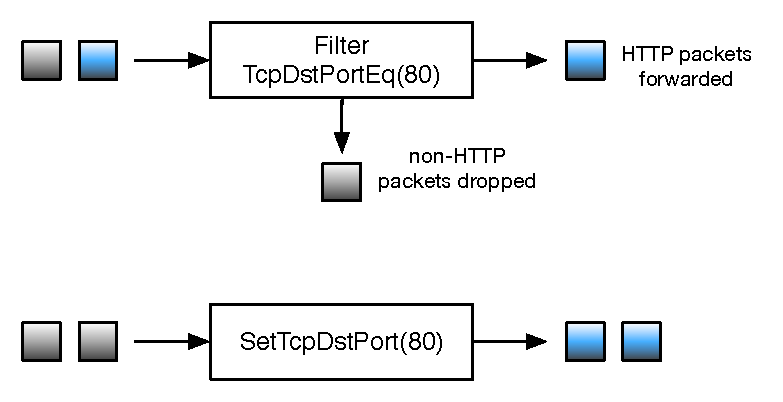
\includegraphics{netkat_policy_building_blocks}
\end{figure}

A filter, shown at the top, takes as input a stream of packets.  Packets that match its criteria are
sent to the next policy, packets that don't match are dropped.  Two special policies, 
\texttt{id} and \texttt{drop}, let through all or no packets respectively.  

A modification, meaning any NetKAT policy beginning with \python{Set}, 
changes packet header values.  In the bottom example, the \texttt{TcpSrcPort} header gets
changed to 80.  This modification happens on a logical copy of the packet.  That means subsequent \texttt{Filters} 
match against the original \netkat{TcpSrcPort} 
value in the header, not the one we just changed it to.  But most of the 
time, you can ignore this subtlety because filters precede modifications.

Modifications to different headers can generally be specified in any order.  If two modifications to the same header 
value occur one after the other, the last one wins.  

You combine these building blocks with \texttt{Seq} and \texttt{Union}.
Here is a \texttt{Seq} of two policies, a filter and a modification.   

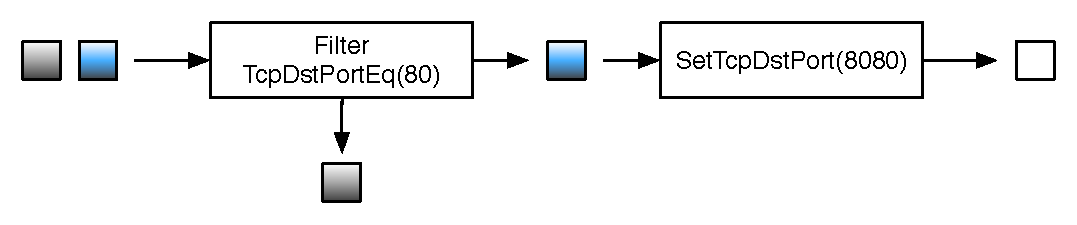
\includegraphics[width=\linewidth]{netkat_policy_combinators_seq}

In sequences, policies
are chained together in a straight line, and packets travel through each of one of the policies in order.  
Combining a filter plus modifications is very common in NetKAT programs, and we generally
use \texttt{Seq} to combine them into a \emph{rule}.  

A rule is like an OpenFlow flow table entry, but with more options.  
If you think about it, a switch receives a huge firehose blast of packets, and you want the switch to 
perform a targeted action on a very small subset of those packets. 
In other words, you want a \emph{filter} and some \emph{actions}.
It's like the MapReduce paradigm, but in reverse order - you first \emph{reduce} the stream to a manageable level,
then \emph{map} the result by performing actions on it.  

With \texttt{Seq}, order matters.  So the rule \texttt{drop >> Filter(EthTypeEq(0x806))} 
drops ALL packets, no matter the type.  
The second filter is never reached.  
In general, putting all the filters before the actions in a sequence chain is the clearest way to write it.

The following principle is a good guideline:  

\begin{principle}
Use \texttt{>>} between filters and all actions.
\end{principle}

Here is a Union of policies.

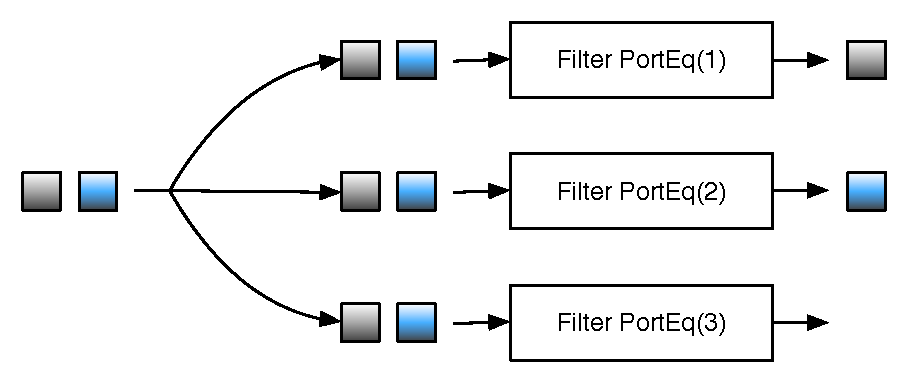
\includegraphics{netkat_policy_combinators_union}

A \texttt{Union} of policies makes logical copies of packets and sends the copy of each packet
through each policy in parallel.  In the above example, the two incoming packets are copied three times, one
for each rule.  In this case, the top filter only forwards a copy of the first packet matching \netkat{PortEq(1)}.
The middle filter only forwards a copy of the second packet  matching \netkat{PortEq(2)}
The bottom filter doesn't forward any packets at all.  

\begin{principle}
Use \texttt{|} between rules that DO NOT overlap.
Use \texttt{IfThenElse} to combine rules that DO overlap. 
\end{principle}

We'll explain \texttt{IfThenElse} in a little bit.  

You might think, ``All that packet copying must be really tough on the switch.''  In fact, all the 
packet copying is conceptual, it doesn't necessarily happen in the switch.  Frenetic turns NetKAT
programs into flow tables, and these flow tables generally work through sophisticated TCAM's, Hash tables,
and pipelines that eliminate actual packet copying.  So don't worry about stringing 20,000 policies
with a \texttt{Union}.  Your switch can handle it.   

\texttt{SetPort} is a little different.  Other modifications like \texttt{SetTcpDstPort} act on a single packet at a time.
A single \texttt{SetPort} is like this - we merely want to change the egress port of the packet itself.  But if 
you want to send it out multiple ports at once, as in flooding, you can send a list of ports to \texttt{SetPort}.

Now let's look at \texttt{Union} and \texttt{IfThenElse}.  
As we have seen in Chapter 2, Union is parallel composition:
we effectively make copies of each packet and apply the rules to each packet.  So in our 
repeater application, the rules are:

\begin{itemize}
  \item \texttt{Filter(PortEq(1)) >> SetPort(2)} Sends traffic from port 1 out port 2 
  \item \texttt{Filter(PortEq(2)) >> SetPort(1)} Sends traffic from port 2 out port 1 
\end{itemize}

A packet cannot match both rules -- in other words, there is no overlap.  So a \texttt{Union} between
these two rules is appropriate.  You make a copy of each packet, send it through each of the rules.  
One or the other will match and send it out the appropriate port, the other will simply drop it.  

Suppose you have two rules:

\begin{itemize}
  \item \texttt{Filter(TcpDstPortEq(80)) >> drop} Drops non-encrypted HTTP traffic 
  \item \texttt{Filter(PortEq(2)) >> SetPort(1)} Sends port 2 traffic out port one.
\end{itemize}

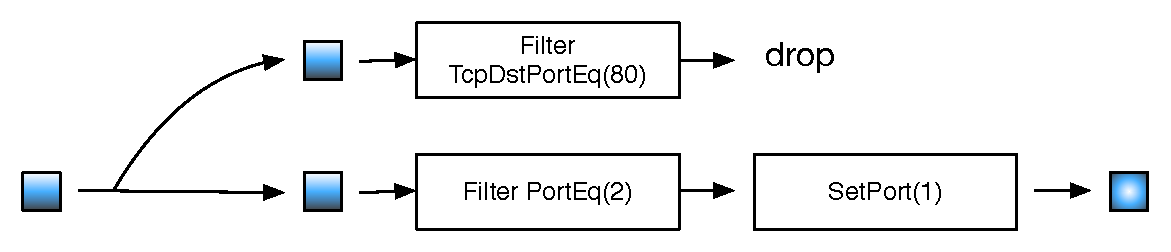
\includegraphics[width=\linewidth]{netkat_overlapping_union}

These two rules overlap.  A packet can both have a TCP destination port of 80 and
arrive on switch 1, port 2.  What happens if we combine them with \texttt{Union}, and a packet
like that arrives at the switch?  The packet will be copied twice, then:

\begin{itemize}
  \item \texttt{Filter(TcpDstPortEq(80)) >> drop} will drop the first copy of the packet 
  \item \texttt{Filter(PortEq(2)) >> SetPort(1)} will send out the second copy to port 1
\end{itemize}

But that's probably not what you intended.  You probably want the HTTP rule to take precedence over the
sending rule.  In such cases,
\texttt{IfThenElse} makes the precedence crystal clear:

\begin{minted}{python}
IfThenElse(TcpDstPortEq(80), drop, Filter(PortEq(2)) >> SetPort(1))}
\end{minted}

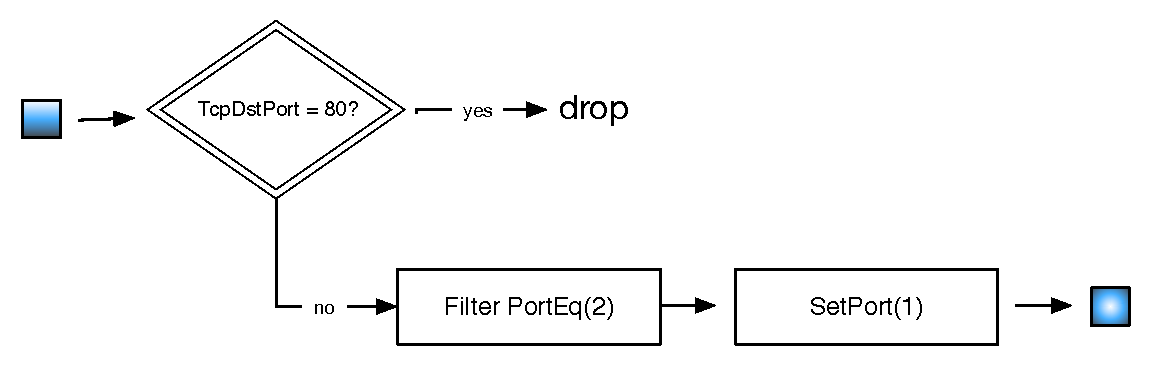
\includegraphics[width=\linewidth]{netkat_overlapping_if_then_else}

The predicate is tested, and if it matches, the first policy is performed, otherwise the second is performed.

That's pretty powerful, and in fact we can write the repeater app to use \texttt{IfThenElse} instead of Union:

\begin{minted}{python}
IfThenElse(PortEq(1), SetPort(2), Filter(PortEq(2)) >> SetPort(1) 
\end{minted}

So why not just use \texttt{IfThenElse} for combining rules all the time?  In a real switch, you might have 
hundreds of non-overlapping rules.  Writing them as:

\begin{minted}{python}
IfThenElse(predicate1), action1, IfThenElse(predicate2, action2, IfThenElse #....
\end{minted}

is doable but a lot more verbose.  It also hides the fact that the rules are non-overlapping, and this is useful
information when rummaging through an SDN app. 

\netkat{IfThenElse} is really syntactic sugar.  The statement:

\begin{minted}{python}
IfThenElse(pred, true_policy, false_policy)
\end{minted}

is just a shortcut for:

\begin{minted}{python}
Filter(pred) >> true_policy | Filter(~ pred) >> false_policy
\end{minted}

but it's a lot shorter and easier to understand, especially for programmers accustomed to seeing If-Then-Else
constructs in other programming languages.

\section{Keeping It Stateless}
\label{section:stateless}

So let's kick it up a notch.  
Our repeater is fast, but pretty static -- it only works with two ports, and only ports that are numbered
1 and 2.
So let's extend our repeater to do two things: 

\begin{enumerate}
\item On connection, read the list of currently available ports and build the initial NetKAT policy accordingly.
\item When ports go up or down, adjust the policy dynamically.
\end{enumerate}

The first task requires us to inquire which ports a switch has.  Frenetic provides a \texttt{current\_switches()}
method that does exactly that.   The best time to call it is on the \texttt{connected()} hook since, at that
point, Frenetic knows the switches and ports out there.

The following code is in \texttt{netkat\_principles/repeater3.py}:

\inputminted{python}{code/netkat_principles/repeater3.py}

\texttt{current\_switches()} is an asynchronous call, meaning you don't get the results immediately.
Instead, we pass a callback procedure named \texttt{handle\_current\_switches}, which Frenetic calls
when the \texttt{current\_switches()} call is complete and has results.  In our first pass, the callback
is just a one line procedure that prints the results to the log (the screen by default).  Although
we could define \texttt{handle\_current\_switches()} outside the \texttt{connected()} method, placing
it inside clarifies the connection between the two.  

So let's start up Mininet with 4 hosts this time:

\begin{minted}{console}
frenetic@ubuntu-1404:~/workspace$ sudo mn --topo=single,4 --controller=remote
*** Creating network
*** Adding controller
Unable to contact the remote controller at 127.0.0.1:6633
*** Adding hosts:
h1 h2 h3 h4
*** Adding switches:
s1
*** Adding links:
(h1, s1) (h2, s1) (h3, s1) (h4, s1)
*** Configuring hosts
h1 h2 h3 h4
*** Starting controller
c0
*** Starting 1 switches
s1 ...
*** Starting CLI:
mininet>
\end{minted}

Start up Frenetic:

\begin{minted}{console}
frenetic@ubuntu-1404:~/workspace$ ~/src/frenetic/frenetic.native http-controller
 [INFO] Calling create!
 [INFO] Current uid: 1000
 [INFO] Successfully launched OpenFlow controller with pid 2035
 [INFO] Connecting to first OpenFlow server socket
 [INFO] Failed to open socket to OpenFlow server: (Unix.Unix_error "...
 [INFO] Retrying in 1 second
 [INFO] Successfully connected to first OpenFlow server socket
 [INFO] Connecting to second OpenFlow server socket
 [INFO] Successfully connected to second OpenFlow server socket
 [INFO] switch 1 connected
\end{minted}

And start up our application:

\begin{minted}{console}
frenetic@ubuntu-1404:~/workspace$ python repeater3.py
No client_id specified. Using 0323e4bc31c94e81939d9f51640f1f5b
Starting the tornado event loop (does not return).
2016-04-12 09:51:14,578 [INFO] Connected to Frenetic - Switches: {1: [4, 2, 1, 3]}
\end{minted}

The \texttt{handle\_current\_switches} callback gets called with a Python dictionary.  
The keys in this dictionary are the datapath ID's (dpid's) of each switch -- in our case, we only have
one switch with a dpid of 1.
The value associated with the key is a list of ports that the switch has operational.  
In this case, we have four ports labelled 1 through 4 (they will be in some random order in the list, as
you see above in \python{[4, 2, 1, 3]}).

Great!  Once we have the list of ports, we can construct policies.  If a packet comes in on port
1, it should be repeated to all the ports that are not 1, e.g. 2, 3 and 4, and so on.   
The NetKAT policy, written out manually, will look like this:

\begin{minted}{python}
Filter(PortEq(1)) >> SetPort(2,3,4) |
Filter(PortEq(2)) >> SetPort(1,3,4) |
Filter(PortEq(3)) >> SetPort(1,2,4) |
Filter(PortEq(4)) >> SetPort(1,2,3)
\end{minted}

Or equivalently with lists:

\begin{minted}{python}
Filter(PortEq(1)) >> SetPort( [2,3,4] ) |
Filter(PortEq(2)) >> SetPort( [1,3,4] ) |
Filter(PortEq(3)) >> SetPort( [1,2,4] ) |
Filter(PortEq(4)) >> SetPort( [1,2,3] )
\end{minted}

A combination of Frenetic and Python lists makes this easy to construct.  
Suppose you have the list named \python{sw} with value 
\python{[1, 2, 3, 4]} from the callback.   The following Python list comprehension:

\begin{minted}{python}
SetPort( [p for p in sw] )
\end{minted}

returns the list:

\begin{minted}{python}
SetPort( [1,2,3,4] )
\end{minted}

Now suppose we're looking only at port 1.  We want all of the ports here 
except 1.  A little tweak to the list comprehension:

\begin{minted}{python}
SetPort( [p for p in sw if p != in_port] )
\end{minted}

Removes the input port from the list, leaving:

\begin{minted}{python}
SetPort( [2,3,4] )
\end{minted}

So here is our repeater that installs an initial configuration.
The following code is in \codefilename{netkat_principles/repeater4.py}:

\inputminted{python}{code/netkat_principles/repeater4.py}

Now it's just a hop, skip and  jump to a fully dynamic repeater.  First we need to capture packets from ports
that we haven't seen yet.  We could write an extremely long filter, filtering out every port that's not on the
list, but since port numbers can be 32-bits long, that's gonna be pretty huge:

\begin{minted}{python}
Filter(PortEq(5, 6, 7, ..., 4294967295) >> SendToController("repeater_app")
\end{minted}

It's easier just to write an overlapping rule.  Recall that \netkat{id} is a filter that matches all packets:

\begin{minted}{python}
id >> SendToController("repeater_app")
\end{minted}

But obviously, this overlaps with the rules for known ports in our repeater.  So we use an \texttt{IfThenElse} to 
resolve the overlap:

\inputminted[firstline=14,lastline=25]{python}{code/netkat_principles/repeater5.py}

We take this opportunity to save the port list in an instance variable \texttt{self.all\_ports}.  This instance variable
is the beginning of a Network Information Base, or NIB -- it encapsulates the known state of the network
at this time.  We're going to see the NIB a lot in future apps.  You can think of our app as a function with the
NIB as input and a NetKAT program as output.  

Now how we do learn about new ports?  A packet arriving at \texttt{pkt\_in} will signal we're seeing a new port.
So suppose we're seeing a packet on port 40.  If you think about, the entire NetKAT program will change from:

\begin{minted}{python}
Filter(PortEq(1)) >> SetPort(2,3,4) |
Filter(PortEq(2)) >> SetPort(1,3,4) |
Filter(PortEq(3)) >> SetPort(1,2,4) | 
Filter(PortEq(4)) >> SetPort(1,2,3)
\end{minted}

to:

\begin{minted}{python}
Filter(PortEq(1)) >> SetPort(2,3,4,40) |
Filter(PortEq(2)) >> SetPort(1,3,4,40) |
Filter(PortEq(3)) >> SetPort(1,2,4,40) | 
Filter(PortEq(4)) >> SetPort(1,2,3,40) |
Filter(PortEq(40)) >> SetPort(1,2,3,4)
\end{minted}

Fortunately, we have all the logic we need in \texttt{self.all\_ports\_policy} already.  We just need
to pass it an amended list of known ports.  Not a problem!

\begin{minted}{python}
  def packet_in(self, dpid, port_id, payload):
    self.all_ports.add(port_id)
    self.update(self.policy())
\end{minted}

What do we do with the packet we just received? 
We could just drop it and hope the host is smart enough to resend it.  But that's not
very hospitable.  

What if we just do a \texttt{pkt\_out} immediately afterward?  After all, we just installed a rule that
will deal with it appropriately, right?

\begin{minted}{python}
  def packet_in(self, dpid, port_id, payload):
    self.all_ports.add(port_id)
    self.update(self.policy())
    self.pkt_out(dpid, payload, ??? )
\end{minted}

There are two problems.  First, it's unclear what the action should be on \texttt{pkt\_out}.  If we send an empty 
list of actions, the OpenFlow switch will interpret it as ``drop the packet.''.  
Second, there's a timing problem.
Even though we just sent a self.update, the call is asynchronous with no response when it's done updating the
OpenFlow flow table.  It could take a microsecond, it could take an hour \ldots we just don't know.  
This timing problem actually can cause more problems.  What if, before the new rules are installed, the 
switch receives 100 more packets?  pkt\_in will be called 100 times, and each time the policy will
be recalculated and sent to the switch.  That could cause major problems since installing switch rules can
be a CPU-intensive process on the switch.

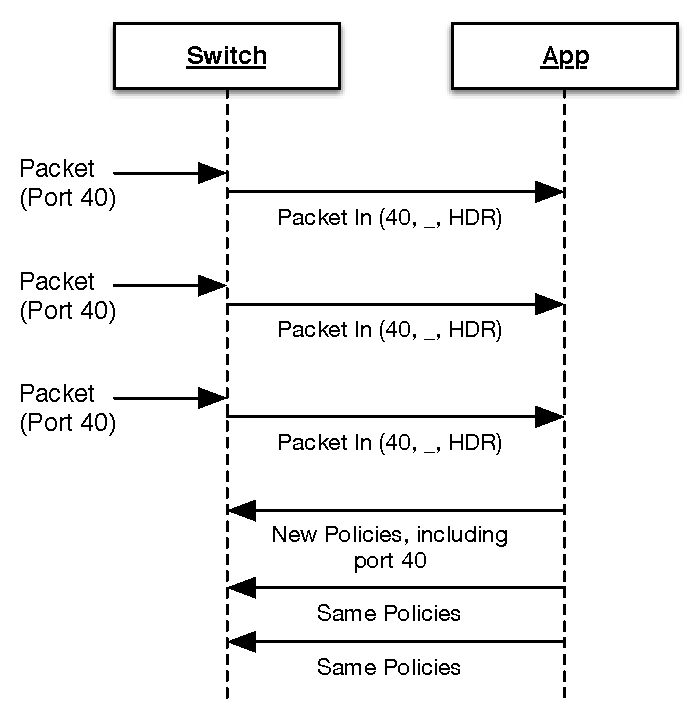
\includegraphics{netkat_policy_timing_problem}

Hence the following principle:

\begin{principle}
When you install a new switch policy, do not assume it'll be installed right away.  
\end{principle}

We can solve this with two quick fixes.  One is to make a quick check that port has not actually be learned yet.
The other is to add actions to pkt\_out that emulate the new rule.  

Here's our final repeater program in \codefilename{netkat_principles/repeater5.py}:

\inputminted{python}{code/netkat_principles/repeater5.py}

In mininet with a simple 4-host topology, we can test our repeater by adding a 5th host and port:

\begin{minted}{console}
mininet> py net.addHost('h5')
<Host h5:  pid=3187>
mininet> py net.addLink(s1, net.get('h5'))
<mininet.link.Link object at 0x7fd432ace810>
mininet> py s1.attach('s1-eth5')
mininet> py net.get('h5').cmd('ifconfig h5-eth0 10.5')
\end{minted}

The new port causes the switch to send an OpenFlow portUp message to our app.  We don't have a handler for
the \texttt{port\_up} hook, so the default message appears:

\begin{minted}{python}
port_up(switch_id=1, port_id=5)
\end{minted}

Back in Mininet, let's try to ping from our new host:

\begin{minted}{console}
mininet> h5 ping -c 1 h1
PING 10.0.0.1 (10.0.0.1) 56(84) bytes of data.
64 bytes from 10.0.0.1: icmp_seq=1 ttl=64 time=996 ms

--- 10.0.0.1 ping statistics ---
1 packets transmitted, 1 received, 0% packet loss, time 0ms
rtt min/avg/max/mdev = 996.738/996.738/996.738/0.000 ms
\end{minted}

Looks good!  A combination of the new packet rules and the \texttt{pkt\_out} 
is sending the packets to the correct place.  

\section{Summary}

In building a dynamic repeater, we have learned the following NetKAT principles:

\setcounter{principle}{0}

\begin{principle}
Keep as much traffic out of the controller as possible.
Instead, program NetKAT policies to make most of the decisions inside the switch.  
\end{principle}

\begin{principle}
Use \texttt{>>} between filters and all actions.
\end{principle}

\begin{principle}
Use \texttt{|} between rules that DO NOT overlap.
Use \texttt{IfThenElse} to combine rules that DO overlap. 
\end{principle}

\begin{principle}
When you install a new switch policy, do not assume it'll be installed right away.  
\end{principle}

And we'll learn a fifth in the next chapter:

\begin{principle}
Do not rely on network state.  Always assume the current packet is the first one you're seeing.   
\end{principle}

These principles are meant as guidelines, not straitjackets.
As we build network applications over the next few chapters, we may find good reasons to violate them 
to achieve shorter code or better modularity.
That's OK. 

Now we have a robust repeater that acts mostly correctly.  There is a still a small timing problem.  If a packet
arrives from port 1 bound for port 40 in that short interval before the rules for port 40 are installed, it
will be copied to ports 2, 3, and 4 but not 40.  There's little we can do in the context of our simple repeater.

But of course, modern network equipment doesn't act like a repeater.  That's 1980's technology!  Repeaters
do a lot of unnecessary packet copying, flooding hosts with packets that are clearly destined for them.  
So our next project will be building an L2 learning switch.  In that context, we'll correct some of the 
remaining timing flaws.  And the result will be much more efficient. 

